\section{Introduction}
Mathematical optimization is one of the pillars of modern machine learning (ML), equipping us with the numerical tools needed to compute parameters for large-scale decision systems. In this work, we focus on \emph{variational inequality problems (VIPs)}—a unifying framework that extends beyond classical loss minimization to encompass min–max optimization, complementarity problems \cite{CottleDantzig1968}, equilibrium computation in games, and general fixed-point formulations. In recent years, VIPs have gained significant traction in ML and data science, especially due to their broad potential applicability in domains where minimizing a single empirical loss is insufficient, with notable examples including generative adversarial networks \cite{goodfellow2014}, multi-agent and robust reinforcement learning \cite{pmlr-v97-zhang19k,rajput2020}, and auction theory \cite{roughgarden2016}.

In practice, many of these tasks reduce to finite-sum formulations, where the objective depends on a large collection of data samples or agents. In such settings, \emph{stochastic gradient methods} have become the workhorse of large-scale learning \cite{Bottou2012,JohnsonZhang2013}. By exploiting the finite-sum structure, stochastic gradient descent (SGD) and its variants replace expensive full-gradient computations with inexpensive updates on a few components, enabling scalability to massive datasets. 

While the theoretical underpinnings of SGD have been extensively studied \cite{Rakhlin2012,ShamirZhang2013,Reddi2018}, much of its practical success can be traced to a handful of seemingly “low-level” heuristics: step-size schedules (constant vs.\ decaying), data ordering (with vs.\ without resampling), and iterate selection (average vs.\ last iterate). To facilitate analysis, the community has typically adopted a \emph{ceteris paribus} perspective—isolating one design choice at a time while holding the rest fixed—an approach that clarifies individual effects but obscures their interaction.

A particularly important example is the use of a \emph{constant step size}. This choice is extremely popular in practice: it makes the algorithm easy to tune, quickly diminishes dependence on initialization, and yields substantial early progress \cite{polyak1992}. Yet it comes with a fundamental limitation: convergence halts at a non-vanishing bias. Even in the simple case of strongly convex problems with a unique solution $x^*$, one typically has
\(
\|x_k - x_*\|^2 = e^{-\rho k}\|x_0 - x_*\|^2 + \text{bias}(\gamma),
\)
where the first term decays exponentially while the residual satisfies $\text{bias}(\gamma) = O(\gamma)$. Thus, in the long run, the iterates stabilize at a point whose distance from the optimum remains on the order of the step size.

To address this issue, practitioners often turn to debiasing heuristics. One such technique, widely adopted in stochastic optimization, is \emph{random reshuffling} (\RRresh), or \emph{without-replacement} sampling, where each data point is used exactly once per epoch. Unlike classical \emph{with-replacement} SGD, which may revisit or skip samples, \RRresh enforces a random full pass that mirrors practical large-scale training \cite{Bottou2012}. Despite the dependence it induces across samples, recent work has established faster convergence guarantees for \RRresh in both minimization and VIPs \cite{Ahn2020,Gurbuzbalaban2021,Mishchenko2020a,Cai2023}, and even bias reduction from $O(\gamma)$ to $O(\gamma^2)$ under suitable conditions.

Orthogonal to reshuffling, another classical idea from numerical analysis has recently re-emerged in stochastic optimization: \emph{Richardson–Romberg} (\RRrom) \emph{extrapolation}. Its principle is simple yet powerful: run the algorithm at two different step sizes and combine their outputs so that the leading bias term cancels. Concretely, whenever the bias admits an expansion of the form $\text{bias}(\gamma) = \Delta \gamma + O(\gamma^{\kappa})$ with $\kappa>1$, running the stochastic approximation at two step sizes gives:
\vspace{-0.5em}\[\text{$x_{\infty}^{\gamma} - x^* = \Delta \gamma + O(\gamma^{\kappa})$ and $x_{\infty}^{2\gamma} - x^* = 2\Delta \gamma + O(\gamma^{\kappa})$.}\vspace{-0.5em}\] 
Extrapolating these iterates then yields \vspace{-0.5em} 
\[
x_{\text{extr}}
= 2x_{\infty}^{\gamma} - x_{\infty}^{2\gamma} - x^*
= \cancel{2\Delta \gamma} - \cancel{2\Delta \gamma} + O(\gamma^{\kappa})
= O(\gamma^{\kappa}). \vspace{-0.5em}
\]
Originally introduced for accelerating discretization schemes in stochastic differential equations \cite{Hildebrand1987,TalayTubaro1990,BallyTalay1996}, \RRrom\ has since been applied to optimization, improving constant-step methods from SGD \cite{Durmus2016,Dieuleveut2020} to Q-learning and two-timescale stochastic approximation \cite{AllmeierGast2024,ZhangXie2024,Huo2024a,Kwon2024}. Despite its conceptual simplicity and empirical success, its theoretical foundations for stochastic VIPs remain nascent \cite{vlatakis2024stochastic}. This raises a fundamental question: 
\begin{equation}
\parbox{35em}{\centering
\textit{What new phenomena arise when these heuristics\\—
\emph{constant step sizes, random reshuffling, and Richardson extrapolation }—\\
interact simultaneously? }
}
\tag{$\bigstar$}
\label{central-question}
\end{equation}
Addressing this question is non-trivial: \RRresh\ produces a biased stochastic oracle whose discrete noise structure lies outside the scope of existing analyses for mainly unbiased \RRrom\ methods \cite{Bach1,Bach2,Mouilines, Vlatakis}. 
\subsection{Our contributions.}
Motivated by this gap, we undertake in this work what is, to the best of our knowledge, the first systematic study demonstrating that these heuristics can be synthesized into a principled algorithmic framework, yielding a composite bias reduction unattainable by any of them in isolation.

\begin{maininformal}
For quasi-strongly monotone smooth VIPs, our combined method (\RRrom$\oplus$\RRresh, Algorithm~X) cancels all lower-order terms in the bias expansion, yielding an asymptotic bias of order $O(\gamma^3)$.
\end{maininformal}

\begin{figure}[ht]
    \centering
    % Left image
    \begin{minipage}{0.48\linewidth}
        \centering
        \includegraphics[width=0.8\linewidth]{iclr2026/placeholder.pdf}
        %\caption*{(a) Bias trajectories for a toy VIP example.}
    \end{minipage}
    \hfill
    % Right image
    \begin{minipage}{0.48\linewidth}
        \centering
        \scalebox{0.45}{% !TEX root = ./iclr2026_conference.tex

\tikzset{every picture/.style={line width=0.75pt}}        

\begin{tikzpicture}[x=0.75pt,y=0.75pt,yscale=-1,xscale=1]


%Shape: Ellipse [id:dp7329906304802944] 
\draw  [fill={rgb, 255:red, 74; green, 144; blue, 226 }  ,fill opacity=0.29 ] (481.22,393.5) .. controls (481.22,299.89) and (557.06,224) .. (650.61,224) .. controls (744.16,224) and (820,299.89) .. (820,393.5) .. controls (820,487.11) and (744.16,563) .. (650.61,563) .. controls (557.06,563) and (481.22,487.11) .. (481.22,393.5) -- cycle ;
%Shape: Ellipse [id:dp14673386188875415] 
\draw  [fill={rgb, 255:red, 126; green, 211; blue, 33 }  ,fill opacity=0.41 ] (537.7,393.5) .. controls (537.7,331.1) and (588.25,280.52) .. (650.61,280.52) .. controls (712.97,280.52) and (763.52,331.1) .. (763.52,393.5) .. controls (763.52,455.9) and (712.97,506.48) .. (650.61,506.48) .. controls (588.25,506.48) and (537.7,455.9) .. (537.7,393.5) -- cycle ;
%Shape: Ellipse [id:dp3138874134344609] 
\draw  [fill={rgb, 255:red, 245; green, 166; blue, 35 }  ,fill opacity=1 ] (568.79,393.5) .. controls (568.79,348.28) and (605.42,311.62) .. (650.61,311.62) .. controls (695.8,311.62) and (732.44,348.28) .. (732.44,393.5) .. controls (732.44,438.72) and (695.8,475.38) .. (650.61,475.38) .. controls (605.42,475.38) and (568.79,438.72) .. (568.79,393.5) -- cycle ;
%Shape: Ellipse [id:dp6951380714624634] 
\draw  [fill={rgb, 255:red, 208; green, 2; blue, 27 }  ,fill opacity=0.73 ] (617.47,393.5) .. controls (617.47,375.18) and (632.31,360.34) .. (650.61,360.34) .. controls (668.91,360.34) and (683.75,375.18) .. (683.75,393.5) .. controls (683.75,411.82) and (668.91,426.66) .. (650.61,426.66) .. controls (632.31,426.66) and (617.47,411.82) .. (617.47,393.5) -- cycle ;

% =============== COLORED POLYLINES WITH STARS ===============

% Green path
\draw [color={rgb, 255:red, 110; green, 192; blue, 19 }, line width=2.25]
  (356,490) -- (341,370) -- (418,243) -- (508,191) -- (594,212) -- (626.22,296.33);
\foreach \p in {(356,490),(341,370),(418,243),(508,191),(594,212),(626.22,296.33)}{
  \node[star, star points=5, draw={rgb,255:red,110; green,192; blue,19},
        fill={rgb,255:red,110; green,192; blue,19}, minimum size=7pt, inner sep=0pt] at \p {};
}

% Blue path
\draw [color={rgb, 255:red, 74; green, 144; blue, 226 }, line width=2.25]
  (356,490) -- (321,336) -- (362,258) -- (424,199) -- (499,157) -- (607,151)
  -- (698,178) -- (728,218) -- (713.68,258.29);
\foreach \p in {  (356,490) , (321,336) , (362,258) , (424,199) , (499,157) , (607,151)
  , (698,178) , (728,218) , (713.68,258.29)}{
  \node[star, star points=5, draw={rgb,255:red,74; green,144; blue,226},
        fill={rgb,255:red,74; green,144; blue,226}, minimum size=7pt, inner sep=0pt] at \p {};
}

% Orange path
\draw [color={rgb, 255:red, 206; green, 131; blue, 13 }, line width=2.25]
  (356,490) -- (388,387) -- (498,266) -- (574,267) -- (601,279) -- (618.6,339.2);
\foreach \p in {(356,490),(388,387),(498,266),(574,267),(601,279),(618.6,339.2)}{
  \node[star, star points=5, draw={rgb,255:red,206; green,131; blue,13},
        fill={rgb,255:red,206; green,131; blue,13}, minimum size=7pt, inner sep=0pt] at \p {};
}

% Red path
\draw [color={rgb, 255:red, 165; green, 6; blue, 24 }, line width=2.25]
  (356,490) -- (420,388) -- (504,346) -- (580,343) -- (641.61,376.61);
\foreach \p in {(356,490),(420,388),(504,346),(580,343),(641.61,376.61)}{
  \node[star, star points=5, draw={rgb,255:red,165; green,6; blue,24},
        fill={rgb,255:red,165; green,6; blue,24}, minimum size=7pt, inner sep=0pt] at \p {};
}

% =============================================================
%
%% Text Node
%\draw (632.38,393.8) node [anchor=north west][inner sep=0.75pt]  [font=\Large,color={rgb, 255:red, 255; green, 255; blue, 255 }  ,opacity=1 ]  {$x_{*}$};
%% Text Node
%\draw (606.03,200.22) node [anchor=north west][inner sep=0.75pt]  [font=\Large,color={rgb, 255:red, 74; green, 144; blue, 226 }  ,opacity=1 ,rotate=-0.45]  {$\mathrm{bias}( \gamma ) =\ \mathcal{O}\left( \gamma \right)$};
%% Text Node
%\draw (671.93,254.71) node [anchor=north west][inner sep=0.75pt]  [font=\Large,color={rgb, 255:red, 100; green, 172; blue, 43 },opacity=1 ,rotate=-25.81]  {$\mathrm{bias}( \gamma ) =\ \mathcal{O}\left( \gamma ^{1.5}\right)$};
%% Text Node
%\draw (598.56,429.08) node [anchor=north west][inner sep=0.75pt]  [font=\Large,color={rgb, 255:red, 208; green, 2; blue, 27 }  ,opacity=1 ,rotate=-0.61]  {$\mathrm{bias}( \gamma ) =\ \mathcal{O}\left( \gamma ^{3}\right)$};
%% Text Node
%\draw (720.43,309.21) node [anchor=north west][inner sep=0.75pt]  [font=\large,color={rgb, 255:red, 231; green, 151; blue, 19 }  ,opacity=1 ,rotate=-60.58]  {$\mathrm{bias}( \gamma ) =\ \mathcal{O}\left( \gamma ^{2}\right)$};
%% Text Node
%\draw (372.38,478.8) node [anchor=north west][inner sep=0.75pt]  [font=\Large,color={rgb, 255:red, 0; green, 0; blue, 0 }  ,opacity=1 ]  {$x_{0}$};

% Text Node
\draw (632.38,393.8) node [anchor=north west][inner sep=0.75pt]  [font=\Large,color={rgb, 255:red, 255; green, 255; blue, 255 }  ,opacity=1 ]  {$x_{*}$};
% Text Node
\draw (606.03,200.22) node [anchor=north west][inner sep=0.75pt]  [font=\large,color={rgb, 255:red, 74; green, 144; blue, 226 }  ,opacity=1 ,rotate=-0.45]  {$\mathrm{bias}( \gamma ) =\ O( \gamma )$};
% Text Node
\draw (665.93,244.71) node [anchor=north west][inner sep=0.75pt]  [font=\large,color={rgb, 255:red, 83; green, 146; blue, 2 }  ,opacity=1 ,rotate=-25.81]  {$\mathrm{bias}( \gamma ) =\ O\left( \gamma ^{1.5}\right)$};
% Text Node
\draw (595.56,429.08) node [anchor=north west][inner sep=0.75pt]  [font=\large,color={rgb, 255:red, 208; green, 2; blue, 27 }  ,opacity=1 ,rotate=-0.61]  {$\mathrm{bias}( \gamma ) =\ O\left( \gamma ^{3}\right)$};
% Text Node
\draw (716.43,301.21) node [anchor=north west][inner sep=0.75pt]  [font=\normalsize,color={rgb, 255:red, 180; green, 117; blue, 0 }  ,opacity=1 ,rotate=-60.58]  {$\mathrm{bias}( \gamma ) =\ O\left( \gamma ^{2}\right)$};
% Text Node
\draw (365.38,478.8) node [anchor=north west][inner sep=0.75pt]  [font=\LARGE,color={rgb, 255:red, 0; green, 0; blue, 0 }  ,opacity=1 ]  {$x_{0}$};

%Straight Lines [id:da7873343135782715] 
\draw    (650.61,393.5) -- (648.05,234) ;
\draw [shift={(648,231)}, rotate = 89.08] [fill={rgb, 255:red, 0; green, 0; blue, 0 }  ][line width=0.08]  [draw opacity=0] (10.72,-5.15) -- (0,0) -- (10.72,5.15) -- (7.12,0) -- cycle    ;
\draw [shift={(650.61,393.5)}, rotate = 269.08] [color={rgb, 255:red, 0; green, 0; blue, 0 }  ][fill={rgb, 255:red, 0; green, 0; blue, 0 }  ][line width=0.75]      (0, 0) circle [x radius= 3.35, y radius= 3.35]   ;
%Straight Lines [id:da8747548930371518] 
\draw    (650.61,393.5) -- (695.72,297.71) ;
\draw [shift={(697,295)}, rotate = 115.22] [fill={rgb, 255:red, 0; green, 0; blue, 0 }  ][line width=0.08]  [draw opacity=0] (10.72,-5.15) -- (0,0) -- (10.72,5.15) -- (7.12,0) -- cycle    ;
\draw [shift={(650.61,393.5)}, rotate = 295.22] [color={rgb, 255:red, 0; green, 0; blue, 0 }  ][fill={rgb, 255:red, 0; green, 0; blue, 0 }  ][line width=0.75]      (0, 0) circle [x radius= 3.35, y radius= 3.35]   ;
%Straight Lines [id:da18150789044644122] 
\draw    (650.61,393.5) -- (713.61,347.16) ;
\draw [shift={(716.03,345.38)}, rotate = 143.66] [fill={rgb, 255:red, 0; green, 0; blue, 0 }  ][line width=0.08]  [draw opacity=0] (10.72,-5.15) -- (0,0) -- (10.72,5.15) -- (7.12,0) -- cycle    ;
\draw [shift={(650.61,393.5)}, rotate = 323.66] [color={rgb, 255:red, 0; green, 0; blue, 0 }  ][fill={rgb, 255:red, 0; green, 0; blue, 0 }  ][line width=0.75]      (0, 0) circle [x radius= 3.35, y radius= 3.35]   ;
%Straight Lines [id:da6863210759512379] 
\draw    (650.61,393.5) -- (665.12,418.22) ;
\draw [shift={(666.64,420.81)}, rotate = 239.59] [fill={rgb, 255:red, 0; green, 0; blue, 0 }  ][line width=0.08]  [draw opacity=0] (10.72,-5.15) -- (0,0) -- (10.72,5.15) -- (7.12,0) -- cycle    ;
\draw [shift={(650.61,393.5)}, rotate = 59.59] [color={rgb, 255:red, 0; green, 0; blue, 0 }  ][fill={rgb, 255:red, 0; green, 0; blue, 0 }  ][line width=0.75]      (0, 0) circle [x radius= 3.35, y radius= 3.35]   ;



% % Central point and labels
% \draw (632.38,393.8) node [anchor=north west][inner sep=0.75pt] [font=\large,color=white] {$x_{*}$};
% \draw (606.03,200.22) node [anchor=north west][font=\footnotesize,color={rgb, 255:red, 74; green, 144; blue, 226 }] {$\mathrm{bias}( \gamma ) =\ O( \gamma )$};
% \draw (671.93,254.71) node [anchor=north west][font=\footnotesize,color={rgb, 255:red, 126; green, 211; blue, 33 }] {$\mathrm{bias}( \gamma ) =\ O\!\left( \gamma ^{1.5}\right)$};
% \draw (598.56,429.08) node [anchor=north west][font=\footnotesize,color={rgb, 255:red, 208; green, 2; blue, 27 }] {$\mathrm{bias}( \gamma ) =\ O\!\left( \gamma ^{3}\right)$};
% \draw (720.43,309.21) node [anchor=north west][font=\footnotesize,color={rgb, 255:red, 231; green, 151; blue, 19 }] {$\mathrm{bias}( \gamma ) =\ O\!\left( \gamma ^{2}\right)$};
% \draw (372.38,478.8) node [anchor=north west][font=\large,color=black] {$x_{0}$};

\end{tikzpicture}}
        %\caption*{(b) Asymptotic neighborhood of $x_k$.}
    \end{minipage}
    \caption{Illustration of bias behavior. 
    \textbf{(a)} Example on a quadratic VIP with $F(x)=\tfrac{1}{N}\sum x^\top A x$ for $N=1000$. 
    Already after the second epoch, the methods clearly separate: 
    \textcolor{blue}{SGD}, \textcolor{green}{\RRresh}, \textcolor{orange}{\RRrom}, 
    and \textcolor{red}{\RRresh$\oplus$\RRrom}. 
    \textbf{(b)} Decomposition of the iterates as 
    $x_k = x_* + C e^{-k} + \text{bias}_{\text{method}}(\gamma)$, 
    illustrating how the asymptotic neighborhood depends on the bias term.}
\end{figure}

\newpage

\begin{figure}[ht]
    \centering
    \scalebox{0.65}{

\tikzset{every picture/.style={line width=0.75pt}} %set default line width to 0.75pt        

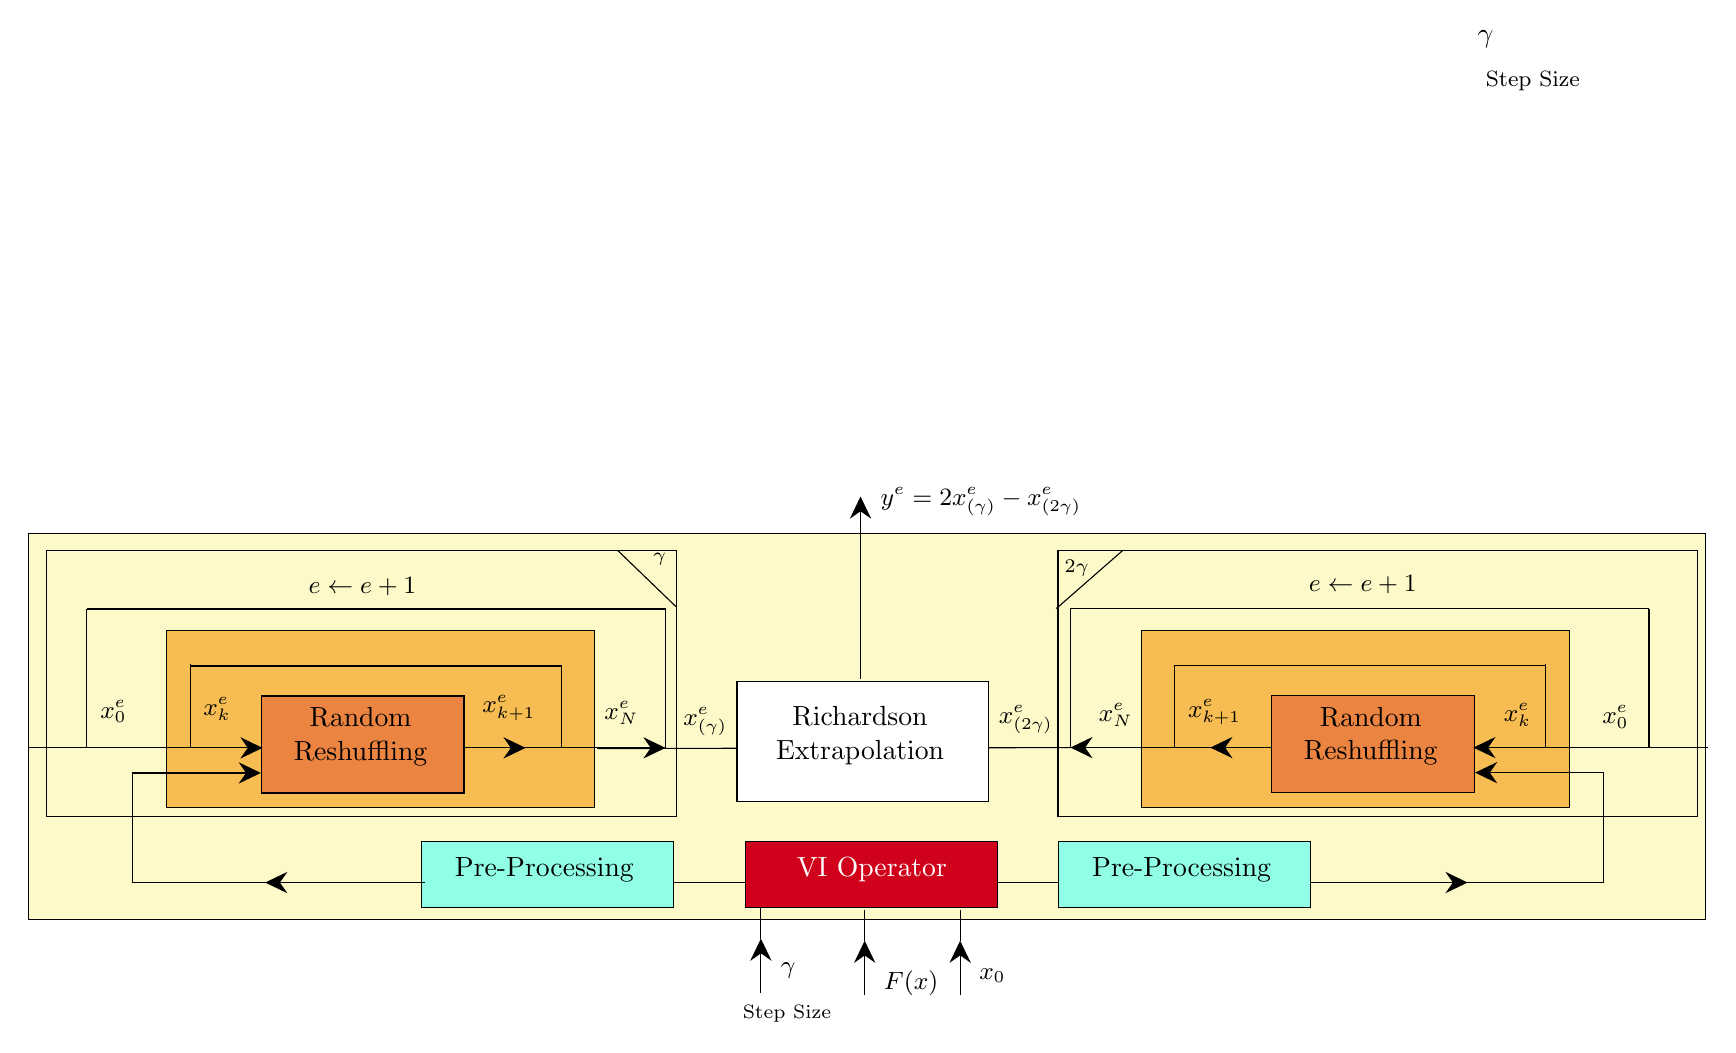
\begin{tikzpicture}[x=0.75pt,y=0.75pt,yscale=-1,xscale=1]
%uncomment if require: \path (0,711); %set diagram left start at 0, and has height of 711

%Shape: Rectangle [id:dp7167201570186642] 
\draw  [fill={rgb, 255:red, 248; green, 231; blue, 28 }  ,fill opacity=0.24 ] (24,362) -- (832,362) -- (832,548) -- (24,548) -- cycle ;
%Straight Lines [id:da5348252051360501] 
\draw    (215.16,530) -- (642,530) ;
%Straight Lines [id:da5870165356755055] 
\draw    (642,530) -- (783.02,530) ;
\draw [shift={(717.51,530)}, rotate = 180] [fill={rgb, 255:red, 0; green, 0; blue, 0 }  ][line width=0.08]  [draw opacity=0] (10.72,-5.15) -- (0,0) -- (10.72,5.15) -- (7.12,0) -- cycle    ;
%Shape: Rectangle [id:dp22967037843062987] 
\draw  [fill={rgb, 255:red, 245; green, 166; blue, 35 }  ,fill opacity=0.71 ] (90.45,408.54) -- (296.62,408.54) -- (296.62,493.84) -- (90.45,493.84) -- cycle ;
%Straight Lines [id:da17785199775015115] 
\draw    (74.14,477.2) -- (133.09,477.2) ;
\draw [shift={(136.09,477.2)}, rotate = 180] [fill={rgb, 255:red, 0; green, 0; blue, 0 }  ][line width=0.08]  [draw opacity=0] (10.72,-5.15) -- (0,0) -- (10.72,5.15) -- (7.12,0) -- cycle    ;
%Shape: Rectangle [id:dp2742561061453428] 
\draw  [fill={rgb, 255:red, 208; green, 2; blue, 27 }  ,fill opacity=0.3 ] (136.49,440.15) -- (233.94,440.15) -- (233.94,486.86) -- (136.49,486.86) -- cycle ;

%Straight Lines [id:da09921992906541832] 
\draw    (102.26,465.12) -- (133.9,465.12) ;
\draw [shift={(136.9,465.12)}, rotate = 180] [fill={rgb, 255:red, 0; green, 0; blue, 0 }  ][line width=0.08]  [draw opacity=0] (10.72,-5.15) -- (0,0) -- (10.72,5.15) -- (7.12,0) -- cycle    ;
%Straight Lines [id:da337709340044827] 
\draw    (234.35,465.12) -- (260.64,465.12) ;
\draw [shift={(263.64,465.12)}, rotate = 180] [fill={rgb, 255:red, 0; green, 0; blue, 0 }  ][line width=0.08]  [draw opacity=0] (10.72,-5.15) -- (0,0) -- (10.72,5.15) -- (7.12,0) -- cycle    ;
%Straight Lines [id:da8354383452527102] 
\draw    (240.28,465.12) -- (281.06,465.12) ;
%Straight Lines [id:da8152793732524597] 
\draw    (281.06,465.12) -- (281.06,425.65) ;
%Straight Lines [id:da7570544004782095] 
\draw    (102.26,465.12) -- (102.26,424.85) ;
%Straight Lines [id:da4721478714710243] 
\draw    (281.06,425.65) -- (102.26,425.65) ;
%Straight Lines [id:da3188806653380546] 
\draw    (281.06,465.12) -- (328.05,465.12) ;
\draw [shift={(331.05,465.12)}, rotate = 180] [fill={rgb, 255:red, 0; green, 0; blue, 0 }  ][line width=0.08]  [draw opacity=0] (10.72,-5.15) -- (0,0) -- (10.72,5.15) -- (7.12,0) -- cycle    ;
%Straight Lines [id:da5695989834818472] 
\draw    (52.27,465.12) -- (102.26,465.12) ;
%Straight Lines [id:da005449392824766197] 
\draw    (52.27,465.12) -- (52.27,398.2) ;
%Straight Lines [id:da5087383745711406] 
\draw    (331.05,465.12) -- (331.05,398.2) ;
%Straight Lines [id:da7805722702952284] 
\draw    (331.05,398.2) -- (52.27,398.2) ;
%Straight Lines [id:da42790020085683145] 
\draw    (52.27,465.12) -- (24.08,465.12) ;
%Shape: Rectangle [id:dp8867101993788168] 
\draw  [fill={rgb, 255:red, 245; green, 166; blue, 35 }  ,fill opacity=0.71 ] (766.71,408.41) -- (560.54,408.41) -- (560.54,493.71) -- (766.71,493.71) -- cycle ;
%Straight Lines [id:da45046936384949954] 
\draw    (783.02,477.06) -- (724.07,477.06) ;
\draw [shift={(721.07,477.06)}, rotate = 360] [fill={rgb, 255:red, 0; green, 0; blue, 0 }  ][line width=0.08]  [draw opacity=0] (10.72,-5.15) -- (0,0) -- (10.72,5.15) -- (7.12,0) -- cycle    ;
%Shape: Rectangle [id:dp8984113920591881] 
\draw  [fill={rgb, 255:red, 208; green, 2; blue, 27 }  ,fill opacity=0.3 ] (623.21,440.01) -- (720.67,440.01) -- (720.67,486.73) -- (623.21,486.73) -- cycle ;

%Straight Lines [id:da49889800256014705] 
\draw    (754.89,464.98) -- (723.26,464.98) ;
\draw [shift={(720.26,464.98)}, rotate = 360] [fill={rgb, 255:red, 0; green, 0; blue, 0 }  ][line width=0.08]  [draw opacity=0] (10.72,-5.15) -- (0,0) -- (10.72,5.15) -- (7.12,0) -- cycle    ;
%Straight Lines [id:da31365561028594713] 
\draw    (622.81,464.98) -- (596.52,464.98) ;
\draw [shift={(593.52,464.98)}, rotate = 360] [fill={rgb, 255:red, 0; green, 0; blue, 0 }  ][line width=0.08]  [draw opacity=0] (10.72,-5.15) -- (0,0) -- (10.72,5.15) -- (7.12,0) -- cycle    ;
%Straight Lines [id:da9666480403965403] 
\draw    (616.88,464.98) -- (576.1,464.98) ;
%Straight Lines [id:da6870758288531431] 
\draw    (576.1,464.98) -- (576.1,425.52) ;
%Straight Lines [id:da13859487218454614] 
\draw    (754.89,464.98) -- (754.89,424.71) ;
%Straight Lines [id:da30734305051591637] 
\draw    (576.1,425.52) -- (754.89,425.52) ;
%Straight Lines [id:da11442520008239165] 
\draw    (576.1,464.98) -- (529.1,464.98) ;
\draw [shift={(526.1,464.98)}, rotate = 360] [fill={rgb, 255:red, 0; green, 0; blue, 0 }  ][line width=0.08]  [draw opacity=0] (10.72,-5.15) -- (0,0) -- (10.72,5.15) -- (7.12,0) -- cycle    ;
%Straight Lines [id:da11238862430956253] 
\draw    (804.89,464.98) -- (754.89,464.98) ;
%Straight Lines [id:da3927723255927097] 
\draw    (804.89,464.98) -- (804.89,398.06) ;
%Straight Lines [id:da17493801390941033] 
\draw    (526.1,464.98) -- (526.1,398.06) ;
%Straight Lines [id:da38944767089549004] 
\draw    (526.1,398.06) -- (804.89,398.06) ;
%Straight Lines [id:da5789729604768556] 
\draw    (298.12,465.45) -- (526.1,464.98) ;
%Straight Lines [id:da5056140478751464] 
\draw    (804.89,464.98) -- (833.08,464.98) ;
%Shape: Rectangle [id:dp6283534568839406] 
\draw   (33,369.87) -- (336.12,369.87) -- (336.12,498) -- (33,498) -- cycle ;
%Straight Lines [id:da7766228141098565] 
\draw    (425,347) -- (425,432) ;
\draw [shift={(425,344)}, rotate = 90] [fill={rgb, 255:red, 0; green, 0; blue, 0 }  ][line width=0.08]  [draw opacity=0] (10.72,-5.15) -- (0,0) -- (10.72,5.15) -- (7.12,0) -- cycle    ;
%Shape: Rectangle [id:dp0677493839993355] 
\draw   (520.12,369.87) -- (828.12,369.87) -- (828.12,498) -- (520.12,498) -- cycle ;
%Shape: Rectangle [id:dp014110378228816445] 
\draw  [fill={rgb, 255:red, 255; green, 255; blue, 255 }  ,fill opacity=1 ] (365.5,433) -- (486.5,433) -- (486.5,491) -- (365.5,491) -- cycle ;

%Shape: Rectangle [id:dp8640505621986145] 
\draw  [fill={rgb, 255:red, 144; green, 255; blue, 229 }  ,fill opacity=1 ] (213.49,510.15) -- (335,510.15) -- (335,542) -- (213.49,542) -- cycle ;

%Shape: Rectangle [id:dp11807891437834184] 
\draw  [fill={rgb, 255:red, 144; green, 255; blue, 229 }  ,fill opacity=1 ] (520.49,510.15) -- (642,510.15) -- (642,542) -- (520.49,542) -- cycle ;

%Straight Lines [id:da6023255336667221] 
\draw    (74.14,477.2) -- (74.14,530) ;
%Straight Lines [id:da047541439752831094] 
\draw    (783.02,477.06) -- (783.02,529.87) ;
%Straight Lines [id:da38440122612945915] 
\draw    (74.14,530) -- (215.16,530) ;
\draw [shift={(138.15,530)}, rotate = 0] [fill={rgb, 255:red, 0; green, 0; blue, 0 }  ][line width=0.08]  [draw opacity=0] (10.72,-5.15) -- (0,0) -- (10.72,5.15) -- (7.12,0) -- cycle    ;
%Shape: Rectangle [id:dp7774128051215404] 
\draw  [fill={rgb, 255:red, 208; green, 2; blue, 27 }  ,fill opacity=1 ] (369.49,510.15) -- (491,510.15) -- (491,542) -- (369.49,542) -- cycle ;
%Straight Lines [id:da048020115234232885] 
\draw    (308,370) -- (336,397) ;
%Straight Lines [id:da22128359563915156] 
\draw    (551.33,370) -- (519.33,398) ;
%Straight Lines [id:da4178126076311651] 
\draw    (427,561) -- (427,584) ;
\draw [shift={(427,558)}, rotate = 90] [fill={rgb, 255:red, 0; green, 0; blue, 0 }  ][line width=0.08]  [draw opacity=0] (10.72,-5.15) -- (0,0) -- (10.72,5.15) -- (7.12,0) -- cycle    ;
%Straight Lines [id:da2712874934584891] 
\draw    (427,543) -- (427,558) ;
%Straight Lines [id:da22537158810197067] 
\draw    (377,560) -- (377,583) ;
\draw [shift={(377,557)}, rotate = 90] [fill={rgb, 255:red, 0; green, 0; blue, 0 }  ][line width=0.08]  [draw opacity=0] (10.72,-5.15) -- (0,0) -- (10.72,5.15) -- (7.12,0) -- cycle    ;
%Straight Lines [id:da17343167705220275] 
\draw    (377,542) -- (377,557) ;
%Straight Lines [id:da5797829827731849] 
\draw    (473,561) -- (473,584) ;
\draw [shift={(473,558)}, rotate = 90] [fill={rgb, 255:red, 0; green, 0; blue, 0 }  ][line width=0.08]  [draw opacity=0] (10.72,-5.15) -- (0,0) -- (10.72,5.15) -- (7.12,0) -- cycle    ;
%Straight Lines [id:da3209997322336591] 
\draw    (473,543) -- (473,558) ;

% Text Node
\draw (147.12,444.5) node [anchor=north west][inner sep=0.75pt]   [align=left] {\begin{minipage}[lt]{53.57pt}\setlength\topsep{0pt}
\begin{center}
Random \\Reshuffling
\end{center}

\end{minipage}};
% Text Node
\draw (382,444) node [anchor=north west][inner sep=0.75pt]   [align=left] {\begin{minipage}[lt]{62.26pt}\setlength\topsep{0pt}
\begin{center}
Richardson\\Extrapolation
\end{center}

\end{minipage}};
% Text Node
\draw (721,118.4) node [anchor=north west][inner sep=0.75pt]    {$\gamma $};
% Text Node
\draw (725,138) node [anchor=north west][inner sep=0.75pt]  [font=\footnotesize] [align=left] {Step Size\\};
% Text Node
\draw (633.84,444.37) node [anchor=north west][inner sep=0.75pt]   [align=left] {\begin{minipage}[lt]{53.57pt}\setlength\topsep{0pt}
\begin{center}
Random \\Reshuffling
\end{center}

\end{minipage}};
% Text Node
\draw (107.08,439.73) node [anchor=north west][inner sep=0.75pt]  [font=\small]  {$x_{k}^{e}$};
% Text Node
\draw (241.59,438.5) node [anchor=north west][inner sep=0.75pt]  [font=\small]  {$x_{k+1}^{e}$};
% Text Node
\draw (300.38,441.53) node [anchor=north west][inner sep=0.75pt]  [font=\small]  {$x_{N}^{e}$};
% Text Node
\draw (57.55,441.12) node [anchor=north west][inner sep=0.75pt]  [font=\small]  {$x_{0}^{e}$};
% Text Node
\draw (157.77,381.59) node [anchor=north west][inner sep=0.75pt]  [font=\small]  {$e\leftarrow e+1$};
% Text Node
\draw (522.12,373.27) node [anchor=north west][inner sep=0.75pt]  [font=\scriptsize]  {$2\gamma $};
% Text Node
\draw (581.57,440.59) node [anchor=north west][inner sep=0.75pt]  [font=\small]  {$x_{k+1}^{e}$};
% Text Node
\draw (733.67,442.41) node [anchor=north west][inner sep=0.75pt]  [font=\small]  {$x_{k}^{e}$};
% Text Node
\draw (538.59,442.4) node [anchor=north west][inner sep=0.75pt]  [font=\small]  {$x_{N}^{e}$};
% Text Node
\draw (781.21,443.59) node [anchor=north west][inner sep=0.75pt]  [font=\small]  {$x_{0}^{e}$};
% Text Node
\draw (433.38,338.53) node [anchor=north west][inner sep=0.75pt]  [font=\small]  {$y^{e} =2x_{( \gamma )}^{e} -x_{( 2\gamma )}^{e}$};
% Text Node
\draw (639.77,380.59) node [anchor=north west][inner sep=0.75pt]  [font=\small]  {$e\leftarrow e+1$};
% Text Node
\draw (338.38,444.53) node [anchor=north west][inner sep=0.75pt]  [font=\small]  {$x_{( \gamma )}^{e}$};
% Text Node
\draw (490.38,443.53) node [anchor=north west][inner sep=0.75pt]  [font=\small]  {$x_{( 2\gamma )}^{e}$};
% Text Node
\draw (223.12,516.5) node [anchor=north west][inner sep=0.75pt]   [align=left] {\begin{minipage}[lt]{72.45pt}\setlength\topsep{0pt}
\begin{center}
Pre-Processing
\end{center}

\end{minipage}};
% Text Node
\draw (323.83,369.96) node [anchor=north west][inner sep=0.75pt]  [font=\scriptsize]  {$\gamma $};
% Text Node
\draw (530.12,516.5) node [anchor=north west][inner sep=0.75pt]   [align=left] {\begin{minipage}[lt]{72.45pt}\setlength\topsep{0pt}
\begin{center}
Pre-Processing
\end{center}

\end{minipage}};
% Text Node
\draw (382.12,516.5) node [anchor=north west][inner sep=0.75pt]  [color={rgb, 255:red, 255; green, 255; blue, 255 }  ,opacity=1 ] [align=left] {\begin{minipage}[lt]{63.95pt}\setlength\topsep{0pt}
\begin{center}
 \ \ VI Operator
\end{center}

\end{minipage}};
% Text Node
\draw (435,571.4) node [anchor=north west][inner sep=0.75pt]  [font=\small]  {$F( x)$};
% Text Node
\draw (385.38,567.53) node [anchor=north west][inner sep=0.75pt]  [font=\small]  {$\gamma $};
% Text Node
\draw (367,588) node [anchor=north west][inner sep=0.75pt]  [font=\scriptsize] [align=left] {Step Size};
% Text Node
\draw (481,570.4) node [anchor=north west][inner sep=0.75pt]  [font=\small]  {$x_{0}$};


\end{tikzpicture}
}
    \caption{Algorithmic Model of \RRresh$\oplus$\RRrom}
\end{figure}

%To the best of our knowledge, this work is the first to demonstrate that these heuristics can be synthesized into a principled algorithmic framework, yielding a composite bias reduction unattainable by any of them in isolation.



% Concretely, whenever the bias expands as $\text{bias}_{}(\gamma) = \Delta \gamma + O(\gamma^{\kappa})$ for some $\kappa>1$,
% then if 
%         $x_{\infty}^{\gamma} - x^* = \Delta\dot\gamma + O(\gamma^{\kappa}), \quad x_{\infty}^{2\gamma} - x^* = \Delta\dot 2\gamma + O(\gamma^{\kappa})$ then extrapolating yields
% $        2x_{\infty}^{\gamma}- x_{\infty}^{2\gamma} - x^* = \cancel{2\Delta \gamma} - \cancel{2\Delta \gamma} + \mathcal{O}\left(\gamma^{\kappa}\right) = \mathcal{O}\left(\gamma^{\kappa}\right) \nonumber
% $

% \begin{eqnarray}
%         x_{\infty}^{\gamma} - x^* = \Delta\dot\gamma + O(\gamma^{\kappa}), \quad x_{\infty}^{2\gamma} - x^* = \Delta\dot 2\gamma + O(\gamma^{\kappa})\\
%         2x_{\infty}^{\gamma}- x_{\infty}^{2\gamma} - x^* = \cancel{2\Delta \gamma} - \cancel{2\Delta \gamma} + \mathcal{O}\left(\gamma^{\kappa}\right) = \mathcal{O}\left(\gamma^{\kappa}\right) \nonumber
% \end{eqnarray}

% \newpage

% Orthogonal to the above, another classical debiasing technique has recently gained traction in stochastic optimization: Richardson–Romberg (RR) extrapolation. Originally developed in numerical analysis to improve the accuracy of discretization schemes [Hildebrand, 1987], RR operates by combining approximations with different step sizes so as to cancel the leading term in the error expansion. The one-step version was introduced to reduce discretization error in Euler schemes for stochastic differential equations [Talay & Tubaro, 1990], later extended to non-smooth settings [Bally & Talay, 1996] and multistep discretizations [Pages, 2007].

% The same idea can be applied to constant-step stochastic gradient methods: if the stationary bias admits an expansion of the form
% x_{\infty}^{\gamma} - x^* = \Delta \gamma + O(\gamma^{\kappa}),
% \quad
% x_{\infty}^{2\gamma} - x^* = 2\Delta \gamma + O(\gamma^{\kappa}),
% then extrapolating yields
% 2x_{\infty}^{\gamma} - x_{\infty}^{2\gamma} - x^*
% = \cancel{2\Delta \gamma} - \cancel{2\Delta \gamma} + O(\gamma^{\kappa})
% = O(\gamma^{\kappa}),
% thereby eliminating the dominant bias term. This simple yet powerful idea has motivated a growing line of work applying RR to stochastic approximation methods, including SGD [Durmus et al., 2016; Dieuleveut et al., 2020; Merad & Gaïffas, 2023; Huo et al., 2024a], Q-learning, and other single- and two-timescale algorithms [Allmeier & Gast, 2024; Zhang & Xie, 2024; Huo et al., 2024a; Kwon et al., 2024].

% Despite this progress, the theoretical understanding of RR in the context of stochastic VIs remains nascent. Prior work has either assumed unbiased stochastic oracles [Bach], or leveraged specific structural properties of the noise [Vlatakis et al.]. Thus, while RR has proven effective in practice and across related stochastic approximation problems, its guarantees for general variational inequalities are still incomplete.

% \newpage


% Orthogonal to the above, there is another folkore from numerical analysis debiasing technique that has become popular in the field of stochastic VIs, the Richardson - Romberg extrapolation. Richardson requires a more refined analysis of the bias of the method, decomposing into a dominant term and some higher order ones, resulting in $\text{bias}_{}(\gamma) = \Delta \gamma + O(\gamma^{\kappa})$
% \begin{eqnarray}
%         x_{\infty}^{\gamma} - x^* = \Delta\dot\gamma + O(\gamma^{\kappa}), \quad x_{\infty}^{2\gamma} - x^* = \Delta\dot 2\gamma + O(\gamma^{\kappa})\\
%         2x_{\infty}^{\gamma}- x_{\infty}^{2\gamma} - x^* = \cancel{2\Delta \gamma} - \cancel{2\Delta \gamma} + \mathcal{O}\left(\gamma^{\kappa}\right) = \mathcal{O}\left(\gamma^{\kappa}\right) \nonumber
% \end{eqnarray}
% Despite the simplicity of the method, the theoretical understanding is nascent. Papers for Richardson explaining the method in minimization (cite Bach) and in VI (Vlatakis). The first analyzed the method with unbiased stochastic oracles, while the second were utilizing specific structure of the noise. 

% Richardson-Romberg (RR) extrapolation is a technique used to improve the accuracy of numerical approximations (Hildebrand, 1987), such as those from numerical differentiation or integration. It involves using approximations with different step sizes and then extrapolating to reduce the error, typically by removing the leading term in the error expansion. The one-step RR extrapolation was introduced to reduce the discretization error induced by an Euler scheme to simulate stochastic differential equation in Talay & Tubaro (1990), and later generalized for non-smooth functions in Bally & Talay (1996). This technique was extended using multistep discretizations in Page`s (2007). RR extrapolation have been applied to Stochastic Gradient Descent (SGD) methods in Durmus et al. (2016), Dieuleveut et al. (2020), Merad & Ga ̈ıffas (2023) and Huo et al. (2024a), to improve convergence and reduce error in optimization problems, particularly when dealing with noisy or high-variance gradient estimates. Recent papers (Allmeier & Gast, 2024; Zhang & Xie, 2024; Huo et al., 2024a; Kwon et al., 2024) consider applications of RR to different stochastic approximation problems with constant step-size, including Q-learning, and single- and two-timescale stochastic approximation.


% To address this issue, practitioners often turn to debiasing heuristics. One such technique, widely adopted in stochastic optimization, is \emph{random reshuffling} (RR), or \emph{without-replacement} sampling, where each data point is used exactly once per epoch. Unlike the classical \emph{with-replacement} variant of SGD—where samples are drawn independently and some may be revisited while others are skipped. RR eliminates this redundancy by enforcing a full pass over the dataset in a random order, closely matching how large-scale training is implemented in practice.
% Despite the dependence it induces across samples within an epoch, recent work has established faster convergence guarantees for RR in both minimization and VIPs \cite{Ahn et al., 2020; Gürbüzbalaban et al., 2021; Mishchenko et al., 2020a; Cai et al., 2023}. Beyond these rate improvements, RR has also been shown to reduce the stationary bias of constant-step methods from $O(\gamma)$ to $O(\gamma^2)$ under suitable conditions.

%To address this issue, practitioners often turn to debiasing heuristics. One such technique, widely adopted in stochastic optimization, is \emph{random reshuffling} (RR)\textendash also known as \emph{without-replacement}, which samples each data point exactly once per epoch. In contrast, the classical \emph{with-replacement} variant of SGD draws each sample independently at every step, so the same data point may be visited multiple times while others are skipped. RR eliminates this redundancy by enforcing a full pass over the dataset in a random order, a procedure that aligns closely with how practitioners typically implement large-scale training, owing to its ease of use and superior empirical performance \cite{Bottou, 2012}. Despite the additional technical challenges introduced by the dependence across samples within an epoch, a series of recent works has established faster convergence guarantees for RR across minimization and variational inequality problems \cite{Ahn et al., 2020; Gürbüzbalaban et al., 2021; Mishchenko et al., 2020a; Cai et al., 2023}. Strikingly, beyond rate improvements, reshuffling has also been shown to mitigate the stationary bias of constant-step stochastic methods, sharpening it from $O(\gamma)$ down to $O(\gamma^2)$ under suitable conditions.

% For example, a particularly important design choice is the use of a \emph{constant step size}. In practice, this setting is extremely popular: it makes the algorithm easy to tune, quickly erases dependence on initialization, and yields rapid early progress \cite{?,?}. Yet it comes with a fundamental limitation: convergence stalls at a non-vanishing bias. Even in the simple case of strongly convex problems with a unique solution $x^$, one typically has
% $\|x_k - x_*\|^2 \;=\; e^{-\rho k}\|x_0 - x_*\|^2 \;+\; \text{bias}(\gamma),$
% with $\text{bias}(\gamma) = O(\gamma)$. Thus, in the long run, the iterates stabilize at a point whose distance from the optimum is of order $\gamma$.
% To facilitate analysis, the leitmotif of the community
% isolates one of these design choices while holding the rest fixed — a ceteris paribus approach that yields valuable but fragmented insights into their impact.
% examines these choices in isolation—adopting a ceteris paribus perspective that clarifies their individual impact but obscures their interaction.



% In practice, many of these tasks reduce to finite-sum formulations, where the objective depends on a large collection of data samples or agents. The success of modern large-scale learning hinges on stochastic methods, which overcome the prohibitive cost of computing full gradients by sampling and updating with only a few components at each iteration.


% Variational inequalities (VIs) form a unifying framework for a wide range of machine learning problems, including adversarial robustness, reinforcement learning, and min–max optimization.

\newpage



% What is the problem?
% Why the problem is important?
% Why the problem is unsolved/history 
% How we resolve it
% Why it was not trivial?


% VI's are important + applications

% Finite-sum: success of Stochastic gradient methods to tame the lack of full-gradient. 
% In the last decades, there is a great effort from the theory community to explain the heuristics that tune the performance of the method in practice.

% The community has explored the effects of an algorithmic heuristic isolated and not the synergy with other common ones. 

% Constant step size: in practice it is used but this leads to bias remaining
% \begin{eqnarray}
%     \|x_k - x_*\|^2 &=& \exp{-\rho k} \|x_0 - x_*\|^2 + \text{bias}(\gamma) \nonumber
% \end{eqnarray}
% The bias in SGD is $\text{bias}(\gamma) = O(\gamma)$. The limit of the iterates could be off the optimal value by a magnitude of order $\text{bias}(\gamma)$. 

% In practice, RR is used because it is beneficial (cite papers). Recently found they provide debiasing $\text{bias}_{\text{RR}}(\gamma) = O(\gamma^2)$.

% Orthogonal to the above, there is another folkore from numerical analysis debiasing technique that has become popular in the field of stochastic VIs, the Richardson - Romberg extrapolation. Richardson requires a more refined analysis of the bias of the method, decomposing into a dominant term and some higher order ones, resulting in $\text{bias}_{}(\gamma) = \Delta \gamma + O(\gamma^{\kappa})$
% \begin{eqnarray}
%         x_{\infty}^{\gamma} - x^* = \Delta\dot\gamma + O(\gamma^{\kappa}), \quad x_{\infty}^{2\gamma} - x^* = \Delta\dot 2\gamma + O(\gamma^{\kappa})\\
%         2x_{\infty}^{\gamma}- x_{\infty}^{2\gamma} - x^* = 2 \Delta\dot\gamma - 2\Delta\dot\gamma + \mathcal{O}\left(\gamma^{\kappa}\right) = \mathcal{O}\left(\gamma^{\kappa}\right) \nonumber
% \end{eqnarray}

% Despite the simplicity of the method, the theoretical understanding is nascent. Papers for Richardson explaining the method in minimization (cite Bach) and in VI (Vlatakis). The first analyzed the method with unbiased stochastic oracles, while the second were utilizing specific structure of the noise. 

% In this work, we ask the question: 
% What is the mutual impact of all the aforementioned heuristics when they are applied simultaneously?

% This questions makes sense and it is non-trivial, as the RR heuristic provides a biased stochastic oracle. Even if Emmanouilidis et al. provide bounds in the second moment, the noise from the stochastic algorithm is discrete and thus direct application of the previous results (Bach, Vlatakis) do not hold. In this work, it is the first time to the best of our knowledge that we present an algorithmic way to combine the heuristics in an effective way for reducing the bias in a composite way. 

% Figure with both plots (left: bias vs step-size, right: 2D plot showing neighbourhoods)

% Algorithm: legend provide details about smoothing noise

% Our contributions:
% - Convergence guarantees for a structured class of non-quasi-monotone problems, establishing exponential convergence up to the bias term
% - Sufficient statistics proving that the average iterate of the algorithm follows a law of large numbers and a corresponding central limit theorem
% - Building upon the aforementioned contributions, we establish an accelerated convergence of the proposed algorithm given the refined bias shown:
% Informal Result

% The first two are preliminaries for establishing the last one, which is the main. 

% From technical perspective, we show Constant step size per epoch the MC is a continuous space homogeneous, Markov Chain. The randomness space is $(U_k, \omega)$, however they are independent between each other and the space is decomposed, where the space of permutations is a redundant MC 

\textit{Paragraph on the Algorithm} We analyze stochastic gradient algorithms that use random reshuffling as the sampling technique for selecting the data and estimating the stochastic oracles of the gradients/operators at them. Specifically, at the start of each epoch $k >0$ a permutation $\omega_k$ of $[n]$ is drawn uniformly at random, specifying an ordering of the data in the dataset for evaluating the stochastic gradients inside the epoch. The algorithm consequently performs the classical update rule of SGD(A) 
\begin{equation}\tag{SGDA-RR}
    x_k^{i+1} = x_k^i - \gamma g(x^i_k; \omega_k^i) \label{SGDA-RR}
\end{equation}
where $g(x_i^k; \omega_k^i)$ is the stochastic oracle evaluated at $x^i_k$ and defined by the corresponding $\omega_k^i$ data point of the dataset. In this work, we allow the stochastic oracle to be either the typical stochastic gradient $g(x_i^k; \omega_k^i) = F_{\omega_k^i}(x_k^i)$ or a smooth version of it [motivated by applications and cite papers here]. 
As a last step, the last iterate of the epoch is set as a starting point for the next epoch and the algorithm reiterates. 
